\chapter{Método}
\label{cap:metodo}

Este trabalho é uma pesquisa aplicada, de abordagem quantitativa e caráter experimental. O método transforma um par de imagens de fluorescência em registros por núcleo, imagens de controle de qualidade e resumos por amostra. O código do pipeline revisado está concentrado em \texttt{pipeline\_melhorado.py}. A implementação é uma alternativa em Python ao algoritmo de referência em MATLAB, desenvolvido por Breno.

\section{Base de imagens e pareamento}

A base contém imagens TIFF relacionadas a núcleos e proteínas de interesse em larvas de \textit{Drosophila melanogaster}. Os arquivos possuem convenções de nome que incluem identificadores da amostra e sufixos de canal, como \texttt{\_z0\_ch00.tif} e \texttt{\_z0\_ch02.tif}. O método normaliza também a variante sem o trecho \texttt{\_z0}. Assim, a chave de uma amostra é a parte do nome anterior ao sufixo de canal.

O pareamento é feito por essa chave, e não pela posição dos arquivos em uma lista. Para cada chave, o manifesto registra os caminhos dos canais de núcleo e proteína ou assinala uma associação incompleta. Essa escolha torna visível qualquer ausência de dado e recupera a amostra cujo nome contém \texttt{Image007}, que não era reconhecida pelo procedimento anterior.

\begin{figure}[htb]
    \centering
    \begin{minipage}{0.47\textwidth}
        \centering
        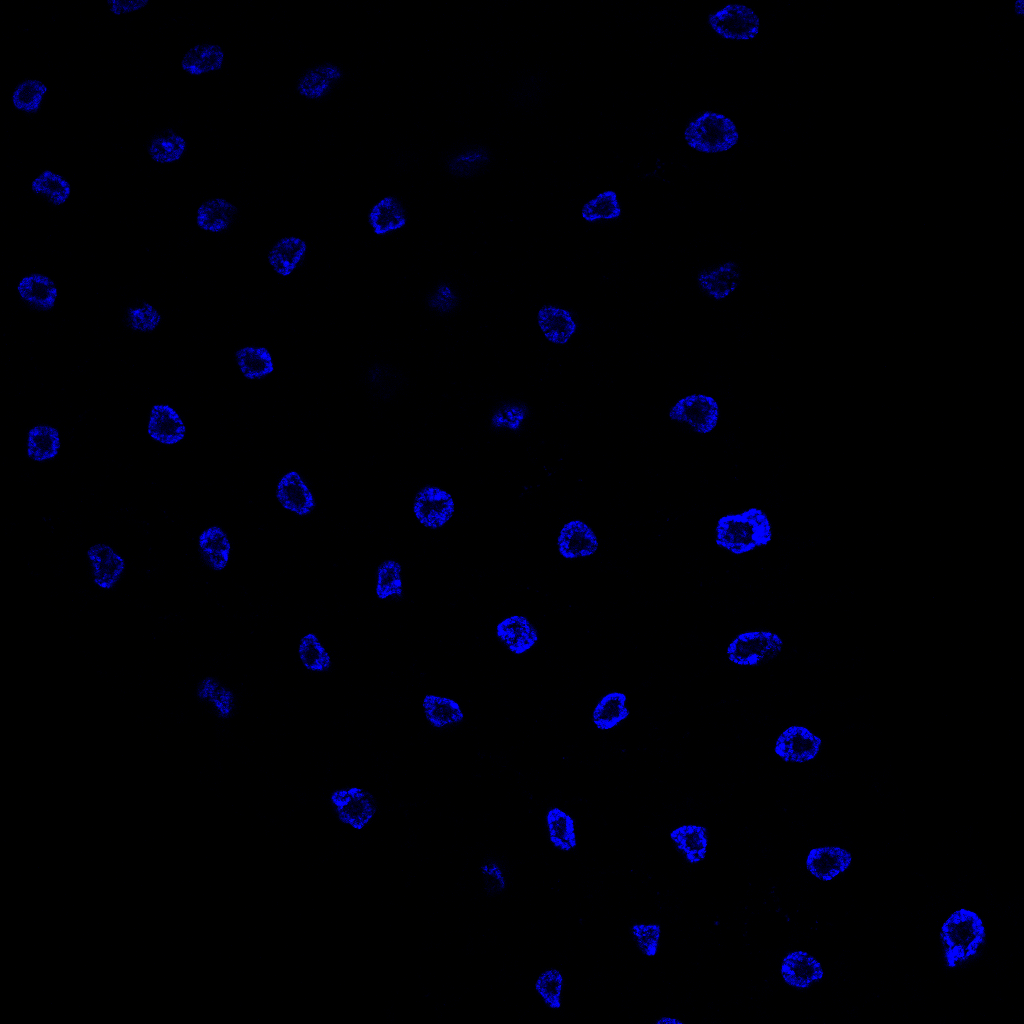
\includegraphics[width=\linewidth]{figs/img_nucleos1.png}

        (a) Canal utilizado para os núcleos.
    \end{minipage}
    \hfill
    \begin{minipage}{0.47\textwidth}
        \centering
        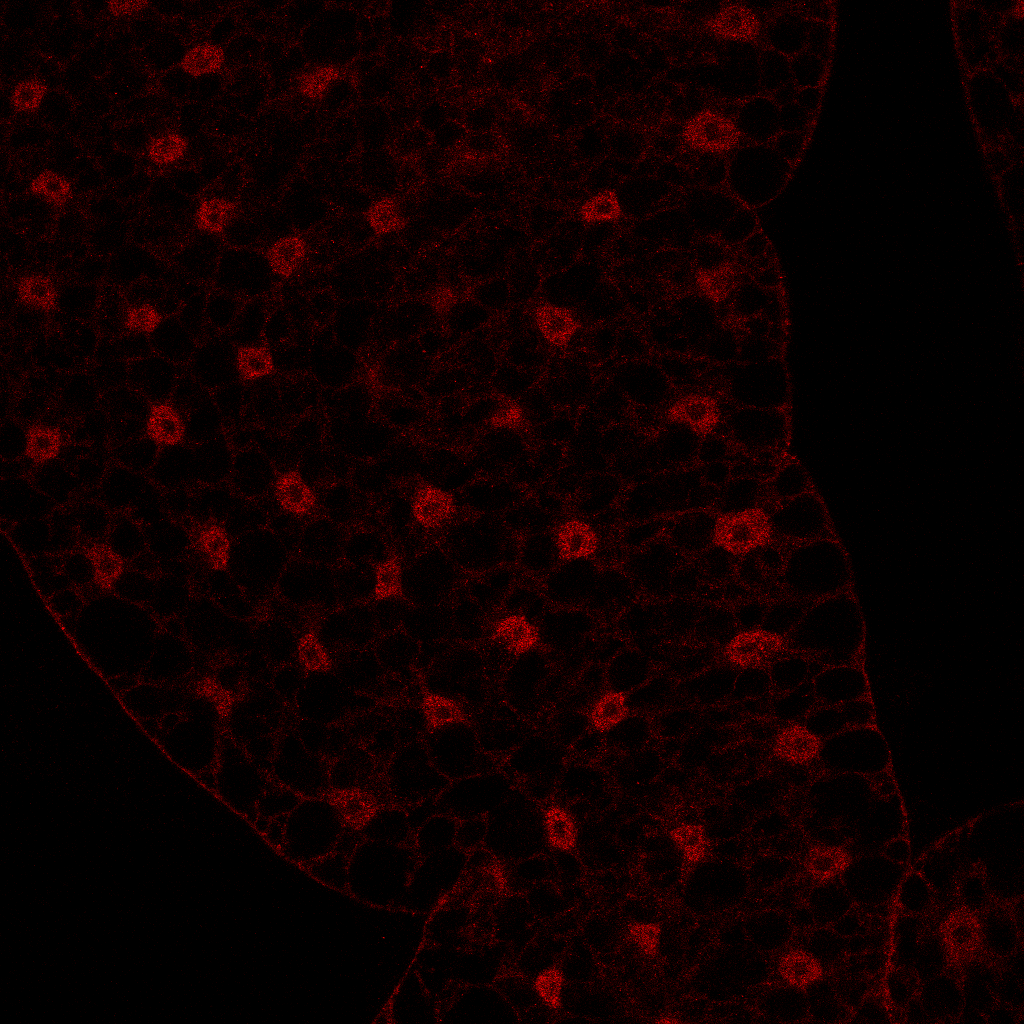
\includegraphics[width=\linewidth]{figs/img_proteina1.png}

        (b) Imagem correspondente de proteína.
    \end{minipage}
    \caption{Exemplo de par de imagens de fluorescência utilizado no pipeline.}
    \label{fig:par-fluorescencia}
    \fonte{Elaborado pelo autor (2026).}
\end{figure}

\section{Pipeline de processamento}
\label{sec:pipeline}

Cada par válido é submetido às etapas descritas a seguir.

\begin{enumerate}
    \item \textbf{Leitura e validação.} As imagens são lidas preservando a profundidade disponível. O algoritmo verifica existência, dimensionalidade, canais solicitados, dimensões espaciais compatíveis e chaves duplicadas.
    \item \textbf{Seleção de canal.} O canal 0 da imagem de núcleos é convertido para matriz de ponto flutuante e utilizado na segmentação. O canal 2 da imagem de proteína é preservado para a quantificação. A visualização normalizada não é usada nos cálculos.
    \item \textbf{Suavização e limiarização.} O sinal de núcleos é limitado ao intervalo de 8 bits, filtrado com Gaussiano de tamanho $5 \times 5$ e desvio-padrão 1,0; em seguida, recebe limiarização binária de Otsu.
    \item \textbf{Limpeza da máscara.} Uma abertura morfológica elíptica de tamanho $3 \times 3$ remove pontos isolados. Um fechamento elíptico de $5 \times 5$ reduz pequenas falhas internas.
    \item \textbf{Identificação de instâncias.} Componentes conectados com conectividade 8 são rotulados. Componentes com menos de 100 pixels são descartados e os identificadores restantes são remapeados para uma sequência contínua.
    \item \textbf{Medição por núcleo.} Para cada rótulo, os pixels internos são usados diretamente para calcular estatísticas do canal de proteína e atributos geométricos.
    \item \textbf{Saídas auditáveis.} O método salva máscara binária, sobreposição colorida, manifesto, configuração e tabelas CSV por núcleo e por amostra.
\end{enumerate}

A Tabela \ref{tab:parametros} sintetiza os parâmetros padrão. Eles são guardados em \texttt{configuracao.json}; portanto, uma alteração de parâmetro não fica implícita no resultado produzido.

\begin{table}[htb]
    \centering
    \caption{Parâmetros padrão do pipeline revisado.}
    \label{tab:parametros}
    \begin{tabular}{|p{0.40\textwidth}|p{0.18\textwidth}|p{0.29\textwidth}|}
        \hline
        \textbf{Parâmetro} & \textbf{Valor} & \textbf{Finalidade} \\
        \hline
        Canal de núcleos & 0 & Sinal empregado na segmentação. \\
        \hline
        Canal de proteína & 2 & Sinal empregado na quantificação. \\
        \hline
        Filtro Gaussiano & $5 \times 5$, $\sigma=1{,}0$ & Redução de ruído antes da limiarização. \\
        \hline
        Abertura / fechamento & $3 \times 3$ / $5 \times 5$ & Limpeza e preenchimento local da máscara. \\
        \hline
        Área mínima & 100 pixels & Remoção de componentes pequenos. \\
        \hline
    \end{tabular}
    \fonte{Elaborado pelo autor (2026).}
\end{table}

\section{Produtos da segmentação}

A Figura \ref{fig:produto-segmentacao} apresenta dois produtos do processamento de uma amostra. A máscara contém somente os núcleos preservados após a limpeza e o filtro de área. A sobreposição colorida é produzida exclusivamente para inspeção visual: ela permite conferir a correspondência espacial entre a imagem e os objetos segmentados, mas não é reutilizada para mensurar intensidade.

\begin{figure}[htb]
    \centering
    \begin{minipage}{0.32\textwidth}
        \centering
        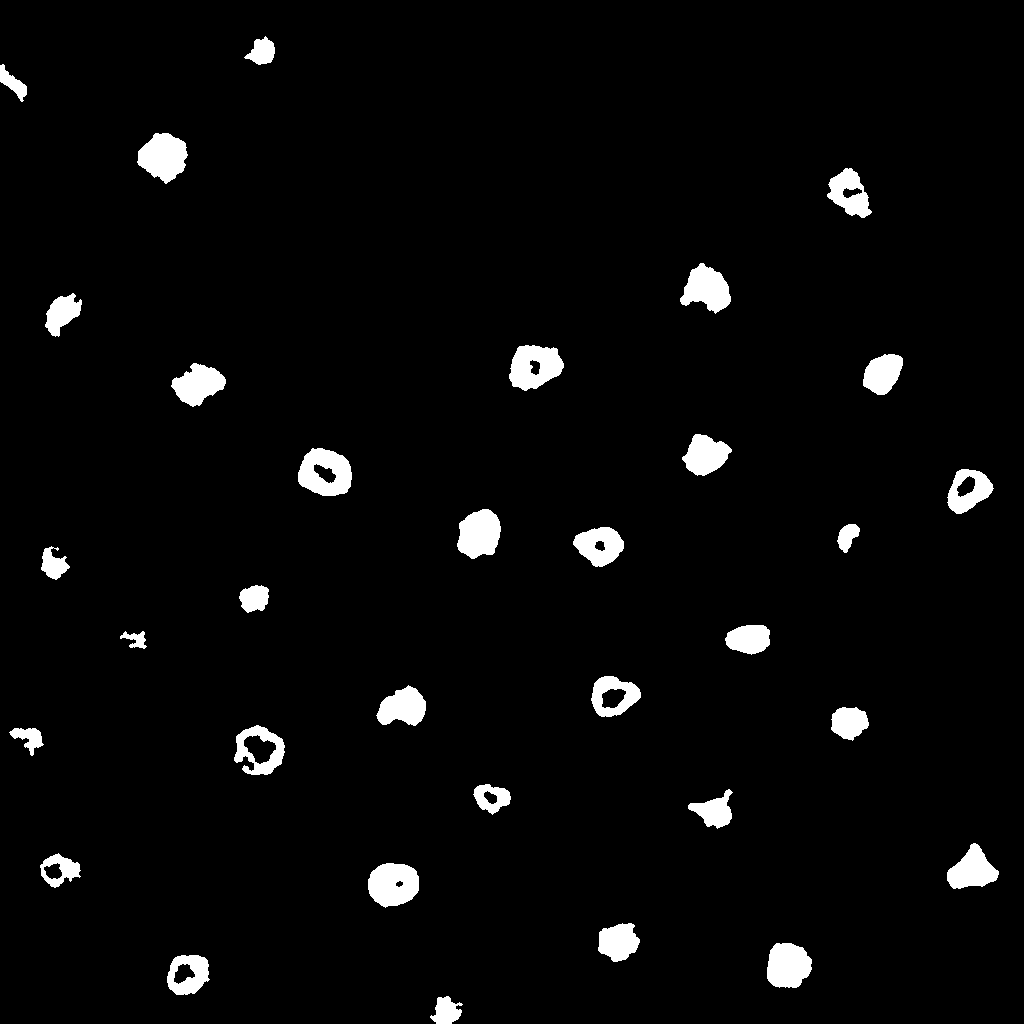
\includegraphics[width=\linewidth]{figs/mascara_exemplo.png}

        (a) Máscara binária.
    \end{minipage}
    \hfill
    \begin{minipage}{0.62\textwidth}
        \centering
        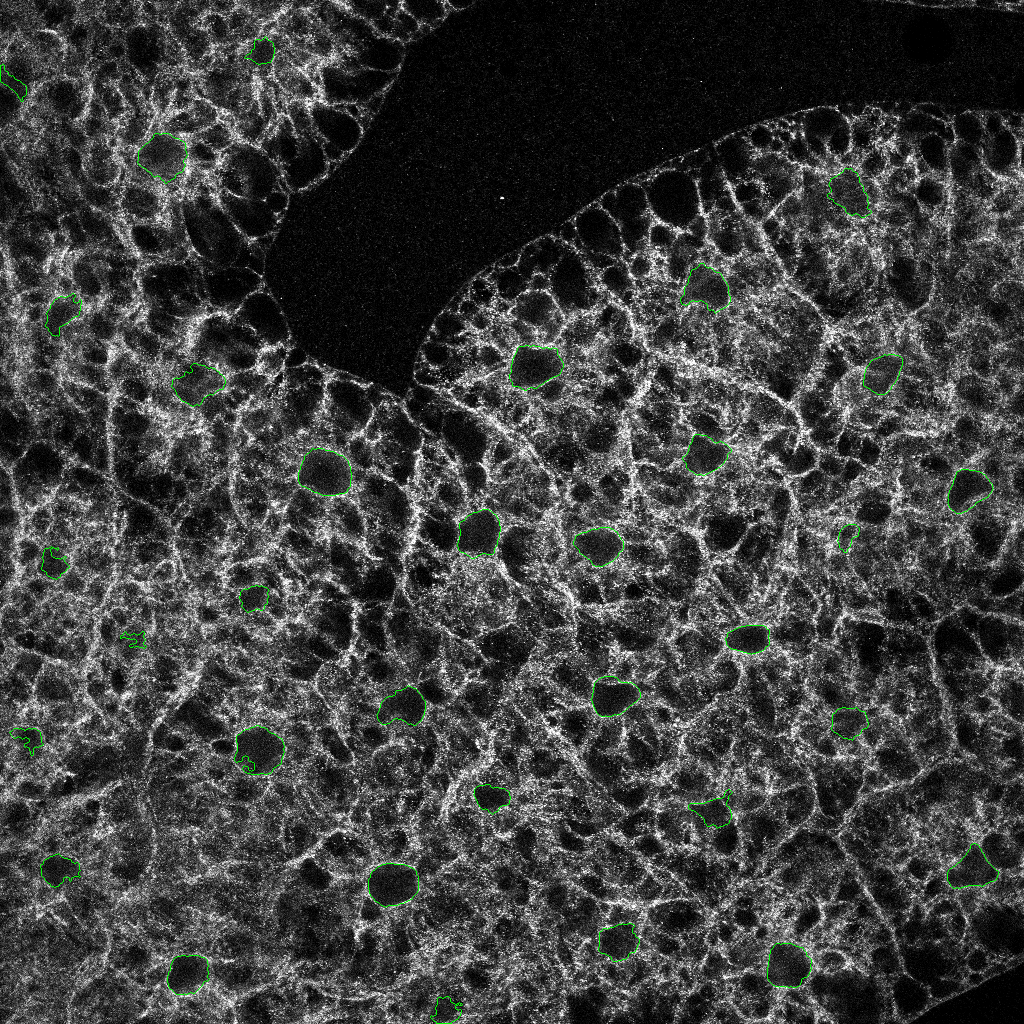
\includegraphics[width=\linewidth]{figs/sobreposicao_exemplo.png}

        (b) Sobreposição de controle de qualidade.
    \end{minipage}
    \caption{Exemplo de produtos gerados pelo pipeline revisado.}
    \label{fig:produto-segmentacao}
    \fonte{Elaborado pelo autor (2026).}
\end{figure}

\section{Medidas extraídas}

Cada núcleo recebe um identificador e um registro contendo área, área espacial quando o tamanho de pixel é informado, centroide, perímetro, raio e diâmetro equivalentes, eixos de elipse, excentricidade e circularidade. Para a proteína são calculadas média, mediana, desvio-padrão e intensidade integrada diretamente sobre os pixels internos. A média de uma amostra é a média das médias individuais dos núcleos; desse modo, imagens com maior número de objetos não dominam a estatística apenas por terem mais pixels.

O arquivo \texttt{resultados\_por\_nucleo.csv} é a saída analítica principal. O arquivo \texttt{resumo\_por\_amostra.csv} contém quantidade de núcleos, área total, limiar de Otsu e média por imagem. O manifesto e o arquivo de configuração completam a trilha de auditoria.

\section{Interface gráfica de revisão}

Além da execução em lote, foi construída uma aplicação web local composta por um cliente React com TypeScript e um servidor FastAPI. O servidor reutiliza as funções de leitura e segmentação do pipeline, executa trabalhos em um conjunto limitado de \textit{workers}, mantém sessões locais e armazena metadados e histórico em SQLite. O cliente permite selecionar as imagens, configurar canais e área mínima, visualizar as camadas de núcleo, proteína e máscara, selecionar objetos e exportar CSV ou JSON.

A edição de contorno recalcula apenas o núcleo modificado, e operações de ocultar, excluir e restaurar são registradas com revisão otimista. Caso duas operações partam de versões diferentes da mesma sessão, a API devolve conflito em vez de sobrescrever silenciosamente uma alteração. A interface também oferece desfazer e refazer. Nomes que indicam imagens derivadas, como máscaras ou sobreposições, geram aviso porque seus pixels podem não corresponder ao sinal bruto.

\section{Critérios de avaliação}

A avaliação operacional foi conduzida por três verificações: (i) execução dos testes de regressão do pipeline e dos testes da API e do cliente; (ii) inspeção visual das máscaras e sobreposições; e (iii) comparação das médias de intensidade por imagem com as saídas do algoritmo de referência em MATLAB. A comparação abrange 204 imagens distribuídas em oito conjuntos experimentais. Para cada imagem são comparadas a média de intensidade do algoritmo de referência e a média obtida pelo pipeline, além da contagem de núcleos. São reportados erro absoluto, erro relativo, proporção de imagens dentro de $\pm 10\%$ e correlação de Pearson. Como os dados disponibilizados para essa comparação são máscaras e imagens de borda derivadas, a análise verifica compatibilidade entre implementações; ela não substitui uma avaliação de acurácia de segmentação contra anotações manuais sobre os TIFFs brutos.
